There are two major sections into which the design solution can be divided. These two sections are data and implementation. The first section, data, takes heavily from last year's report, as there were only minor changes. 

\subsection{Data}

The data section of our design solution includes anything relevant to data, including collecting, storing, and accessing the data.
\subsubsection{Collecting Data}
Initially we had two candidates for the primary source of obtaining all NBA player and team related statistics. These two sources were: 
\begin{itemize}
\item stats.nba.com
\item basketball-reference.com
\end{itemize}
Both sources contained similar amounts of information on player matches, player season averages, teams, matches, with basketball reference being slightly more detailed in aspects such as player season averages and player matches. While both sources were credible, we decided to use stats.nba.com as the primary source as we felt the official statistics platform of the NBA would have more reliable data compared to one that is not affiliated.

The collection of data from stats.nba.com is done by finding a webpage with pertinent data, scraping that data using Python, and storing it in a MySQL database. We automated the process of scraping the data by writing python scripts that iterate through all web pages of a specified type and searching through HTML tags to retrieve the desired data. This usually entails locating an HTML table, iterating through its rows and columns, and retrieving stats for points, assists, rebounds, etc. The two fundamental tools used in the scraping process were the python libraries:
\begin{itemize}
\item BeautifulSoup4
\item Selenium
\end{itemize}

BeautifulSoup allows for objectification of HTML tags on a web page such that can be accessed  through Python and Selenium automates the usage of a chosen browser. While, in most cases, BeautifulSoup alone would be enough to simply access the HTML elements of a given web page, stats.nba.com generates all of the data that we need through JavaScript. This causes a problem for us, as BeautifulSoup has a feature to wait until a page has fully loaded, but this does not take into account JavaScript components. When Selenium is used to automate browser control, we can specify that a page is not fully loaded until all of its JavaScript components have fully loaded.


\subsubsection{Storing Data}
On the topic of data storage we, once again, had 2 major choices with their respective advantages and drawbacks. The methods of storing data were:
\begin{itemize}
\item local database, local files
\item remote database
\end{itemize}
The method of using a local database or local files was enticing due to the lack of potential bottleneck associated with the connection bandwidth of a remote database. However, we knew that the convenience afforded by using a remote database would be more beneficial in the initial data collection process.

While employing the methods to collect data from stats.nba.com, we knew that there existed the potential for database schema changes as we discovered what was available to us and what we wanted to collect. In the case of a local database this would have created an inconsistency in the local copies for each group member. 

Another benefit to using a remote database, at least initially in the data collection process, is the ability to update one persistent database in parallel. Which is to say, multiple people can be using to multiple tables at once to insert or delete entries as more data was collected or data was determined to be obsolete. This convenience is more beneficial than the cost of overhead in using a remote database for as long as data is still being collected. 


\subsubsection{Accessing Data}

Since we decided to employ a remote database for data storage each group member is able to access the data through SSH. Each member has their own credentials through which they can access they database from any location that has access to the internet.


\subsection{Implementation}
We began designing the software architecture before finishing the aforementioned database design. Our initial design was a single neural network that took in, as input, all of the stats of every active NBA player. Additionally, it had an extra input for every player which was set to 1 if the player was playing tonight, and 0 if the player was not. The goal of this neural net was to output the best lineup for the competition. A block diagram of this system can be seen in Figure \ref{fig:first_iteration}.
\begin{figure}[ht]
    \centering
    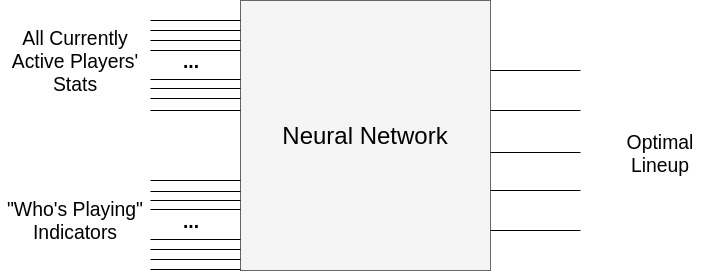
\includegraphics[width=0.75\textwidth]{figures/first_iteration}
    \caption{First design iteration}
    \label{fig:first_iteration}
\end{figure}
 
After discussing this design within our group, and with our supervisor, we realized it had some limitations, listed below. First, this system would only use data from active players. This was not taking advantage of the many decades of basketball data that we had access to. Second, it would also likely require a massive amount of data to be able to learn properly. This is because, generally, the amount of data required to learn adequately is correlated with the complexity of and number of inputs. Third, there would be many unused inputs each time the net is used. Since there are usually only about four NBA games each night, there are only about 80 players active on a single night. There are about 500 total active players, which means that there would be about 420 "unused" inputs. Although this is not explicitly a problem, it makes it seem like there would be a better way to structure the design. The final limitation of the initial neural network that we thought of was that it would be prone to discover "bad" correlations. 
%WEAK%
Since the net only knows which players are playing, and not on which team, it would be bound to find correlations between players that are not playing against each other. To explain, say that NYK is playing against BOS in one game, and GSW is playing against CLE in another. The neural network may find a relationship between someone on BOS and on GSW, even though they are not playing against each other, and games are independent.
%WEAK%
Taking these limitations into account, we designed an improved architecture that was more flexible and required less data to train. We decided on a three step system, of which only one of the steps would involve machine learning, to start. The first system is used to calculate players' scores, the second system uses these as inputs to a neural network to find good players, and the third system selects optimal lineups. An overview of this software architecture can be seen in Figure \ref{fig:second_iteration}.
\begin{figure}[ht]
    \centering
    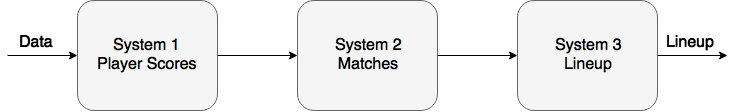
\includegraphics[width=0.85\textwidth]{figures/second_iteration}
    \caption{Redesigned System Architecture}
    \label{fig:second_iteration}
\end{figure}

These three systems will now be looked at in detail.

\paragraph{System 1: Calculating Player Scores}\mbox{}\\
The first step of the design solution is to calculate a score for each player who has played in the NBA. This score is ideally supposed to be a representation of how good the player is, "in a vacuum". That is to say, how well a player will perform if we ignore the match-specific variables like who is on his team, or who he is playing against. Getting a score that represents this is not an exact science. We were initially going to use player rankings given by experts, but could not find historical data for this. Thus, we knew we had to come up with a system of our own to generate these scores. Since we wanted to spend more time focusing on the second system (NN), we decided to initially use a simple equation here based on the player's season statistics, as opposed to something like a neural network. The first equation we decided to use was actually the points system for calculating fantasy basketball scores on FanDuel, seen in Figure \ref{fig:comp_lineup}. We postulate that there is a clear correlation between the amount of fantasy points a player would get, and how good of a player they are. Although this is a simplification, it is a good starting point, and due to the modularity of our design, it can be easily changed and validated on. We then calculated two different types of this score for each player: a short term, and a long term. The short term took the average score of the last n (chosen as 5) games. The long term score took the player's score for their previous season. In the case where it was a player's first season, it took his current season's score so far.
\begin{figure}[ht]
    \centering
    \includegraphics[width=0.5\textwidth]{figures/player_scores}
    \caption{Player scores system}
    \label{fig:player_scores}
\end{figure}
%TODO fix this graphic (it isn't right)
\paragraph{System 2: Matches Neural Network}\mbox{}\\
The scores for every player, obtained in the first step, are then used as inputs for the matches NN. The matches neural net puts two teams of players, each represented by a score, "against each other". That is to say, the first fourteen inputs are used for seven of Team A's players (short term and long term score each), and the next fourteen are used for seven of Team B's players. We selected seven as a compromise between being too restrictive (not all teams have many active players in each position), and getting enough data. The players on each team are ordered by their basketball position. The basketball positions given by our source are guard (G), forward (F), and center (C). As not each team plays the same amount of players in each position, we had to determine what a representative combination of the above positions would look like, which will be discussed in the Data Results section. Ultimately, we decided that a representative set for which we had data would be one center (first input), two guards (second and third inputs), and two forwards (fourth and fifth inputs).\\
The output of the net is a "fantasy game score" for each player. The idea behind this NN is that, since all basketball matches follow the same rules, with the only (or at least most impactful) variable being who is playing on each team, we can train this net on every match that has happened in the past 50 years, and still use it on matches today. This net has a minimal amount of inputs, none of which will be unused. This means it needs less data to train successfully. This design can be seen in Figure \ref{fig:neural_network_full}.

\begin{figure}[ht]
    \centering
    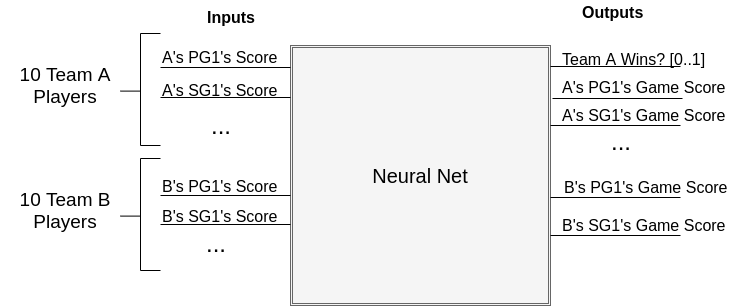
\includegraphics[width=0.6\textwidth]{figures/neural_network_full}
    \caption{Desired complete matches neural network}
    \label{fig:neural_network_full}
\end{figure}

Initially, this network was set to only predict the team that won or lost, and not the game scores of the players. This first prototype was thus not applicable for fantasy basketball, but was used to become familiar with TensorFlow and best practices. We experimented with different input features to see how they impacted the accuracy of the network. In the end, with these ordered positions, the network reached a 63\% prediction accuracy. We did not spend much time attempting to increase this value, as it was an aside from our main goal, predicting lineups.


\paragraph{System 3: Choosing Lineups}\mbox{}\\
The choosing lineups system is the system that takes the player game scores, salaries, and positions of each player in tonight's games, and outputs lineups that optimize the predicted scores. This problem was similar to a backpack problem, but with more constraints. We selected the python library PuLP as the tool to use to solve this constraint problem, and found it to be quite effective. As well, we were able to use this system to generate multiple lineups by applying Gaussian noise to the players' scores before passing these to the system.
%TODO stephen write here about detailed implementation. need figure.

\paragraph{Cross Validation \& Testing}\mbox{}\\
In order to properly test this system, we needed to define a success metric, or a way of measuring how "good" the system was. Ideally, this metric would be profitability, but this was not possible without the historic competition data. Instead, we used a heuristic which is given in Equation \ref{eq_heuristic}

\begin{equation}
Performance = \frac{Maximum Theoretical Lineup Score}{Actual Score of Predicted Lineup}
\label{eq_heuristic}
\end{equation}

This formula yielded around 60\% with random choices between the top seven players on each time. In order to determine what percentage needed to be reached to be profitable, we examined current competitions, and found an effective rule. A system was profitable in most of these competitions when the score reached 80\% of the maximum theoretical score. Figure \ref{fig:80pRule} shows this relationship, where the last winning score is roughly 79\% of the maximum.\\
\begin{figure}[ht]
    \centering
    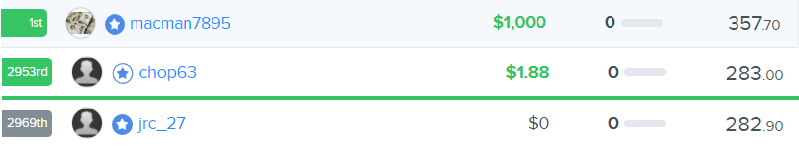
\includegraphics[width=0.6\textwidth]{figures/winningvslosing}
    \caption{Scores for best lineup and barely profitable lineup}
    \label{fig:80pRule}
\end{figure}
In order to increase our performance, we began to train the network. In doing so, we realized that one of the limitations of training and attempting to cross-validate the hyperparameters was the computational time. Thus, we rented a remote computer with a powerful GPU, and changed our machine learning code to be optimized for a GPU. The service we used was called Paperspace, and it was chosen for its low hourly rates with no commitment requirement. We ran cross-validation on Paperspace, and were able to increase this metric over time to 82\% - just above the profitability line. Thus, we began testing in actual competitions; the results of doing so will be discussed in the implementation results section below.

\subsection{Results and Discussion}
There are two types of results that will be given in this report. The first are those related to how much data was scraped from our source, or generated, and the second is related to the success rate of the neural network.

\subsubsection{Data Results}
We managed to scrape, collect, and otherwise compute a significant amount of data to be stored in our database. We were able to gather all data for every basketball game since 1979. We have data for 42000 matches, 10000 player-seasons (unique players for a specific season), 2000 players, and 36 teams, including some that are no longer active. For each match, there are about 15 players with statistics for that match. This is entered in our "player matches" table, and we currently have data in this table for about 25\% of matches. This corresponds to 250,000 entries, and yields about 13000 inputs for our neural net. However, the different architectures which have been presented all impose different constraints on the inputs themselves. For example, the neural network with ordered player scores shown in Figure \ref{fig:neural_network_ordered} requires the match input to have both teams with at least the minimum number of  players (7 in this instance). The neural net with players ordered by position has even more constraints. Not only does it require a minimum number of players per team, but also it needs a minimum number of players per \textit{position}. When performing an analysis on the different player positions per lineup, we found significant variation between teams. This was complicated even further as some players played multiple positions, denoted by two positions separated by a hyphen. For example, the position "F-G" meant that the player could either play a forward or a guard. We found 21 possible combinations of these positions that teams could play. As an example, playing "C, G, G, F, F, C-F" could be a single combination, whereas "F-G, C, C-F, F, F, G, G" could be another. We found that none of the possible 21 combinations had enough data to train our neural network on. Even our initially designed input format of requiring two guards, one center, and two forwards per team (meaning only five inputs per team) caused roughly 21\% of inputs to be discarded, simply because these inputs did not meet the criteria of having these specific numbers of players in each positions.

To avoid losing significant amounts of input data due to constraints, we simplified our input scheme by combining the multi-position players with the single-position players. Our methods of combining these players is shown in Figure \ref{fig:distributionAfterCombination}. Note that the first combination has zero centers (hence no blue bar). In using this scheme, we were able to reduce the amount of lost data to a mere 11\%.

\begin{figure}[ht]
    \centering
    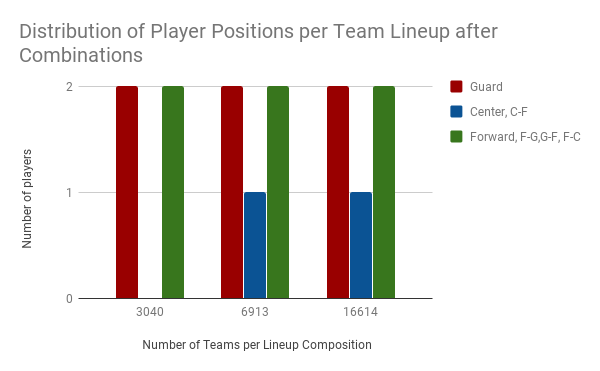
\includegraphics[width=0.75\textwidth]{figures/distributionAfterCombination}
    \caption{Team Compositions by Player Positions After Combinations}
    \label{fig:distributionAfterCombination}
\end{figure}

\subsubsection{Implementation Results}
As mentioned in the description of the neural network in the implementation section, we went through a few different architectures. The final three-system architecture will be the only one discussed in this section, as it is the only one used to enter real competitions. For the results of the earlier architectures, please see our report from the previous term.  Note that these results are on the cross-validated version of the neural network, with two hidden layers, 128 hidden nodes per layer, and a learning rate of 0.01. Furthermore, all accuracy results were obtained by using 70\% of the input data to train the network, and 30\% to test.\\

After cross-validating the system, and entering the first lineups into competitions, we realized we had some overlooked issues. First, the database was not updated, meaning that the short-term scores of each player were actually scores from months ago. Second, we found that we were accidentally ignoring one or two games per night, due to a bug in our code. Thus, our output was only predicting on the other games. Third and finally, we found that many of our selected players would actually not end up playing that night, resulting in zero points. This third issue proved the most challenging to tackle. Although we checked for injuries, we did not perform any more thorough check, and the fantasy website lists all players. Initially, we hoped that we could code something to solve this issue, but we quickly learned that this was not feasible. Ultimately, before submitting each lineup, it is an important step for the user to search NBA news about the player. Sometimes players do not play for personal issues, or because they were only temporarily playing in the spot of another player. We added an option for our system to ignore certain players, for these cases. After solving these issues, we continued entering competitions. To our surprise, the system was somewhat successful. Figure \ref{fig:win_record} are screenshots of the competition summaries for all of the competitions we played in where all of our players played.
\begin{figure}[ht]
    \centering
    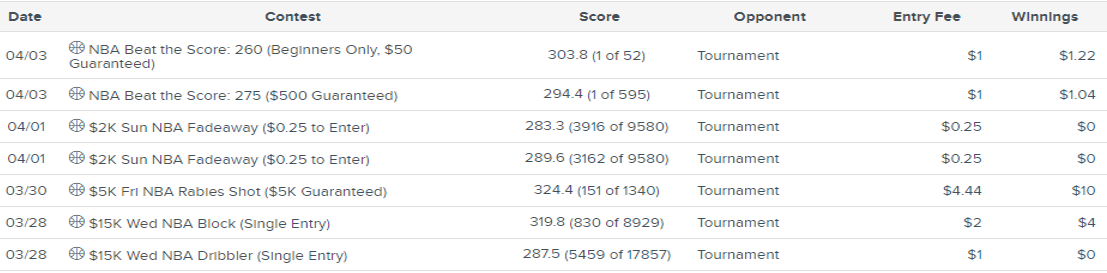
\includegraphics[width=0.6\textwidth]{figures/fanduel_comp}
    \caption{Competition record for submitted lineups}
    \label{fig:win_record}
\end{figure}
One can see that we are overall profitable, but not reliably so, and on a small dataset. When examining the lineups in detail, one can make some interesting observations. For instance, sometimes the network was able to make good predictions that were missed by other competitors. For each player selected, at the end of the competition, a value is given that shows what percentage of other competitors also selected that player. In our best lineup, our players were picked on average 7.5\% by others. The nearest competitor's players averaged a 27\% pickrate. One lineup containing these picks can be seen in Figure \ref{fig:good_picks}. Note that a typical score value for a player with a \$5000 salary is about 15.

\begin{figure}[ht]
    \centering
    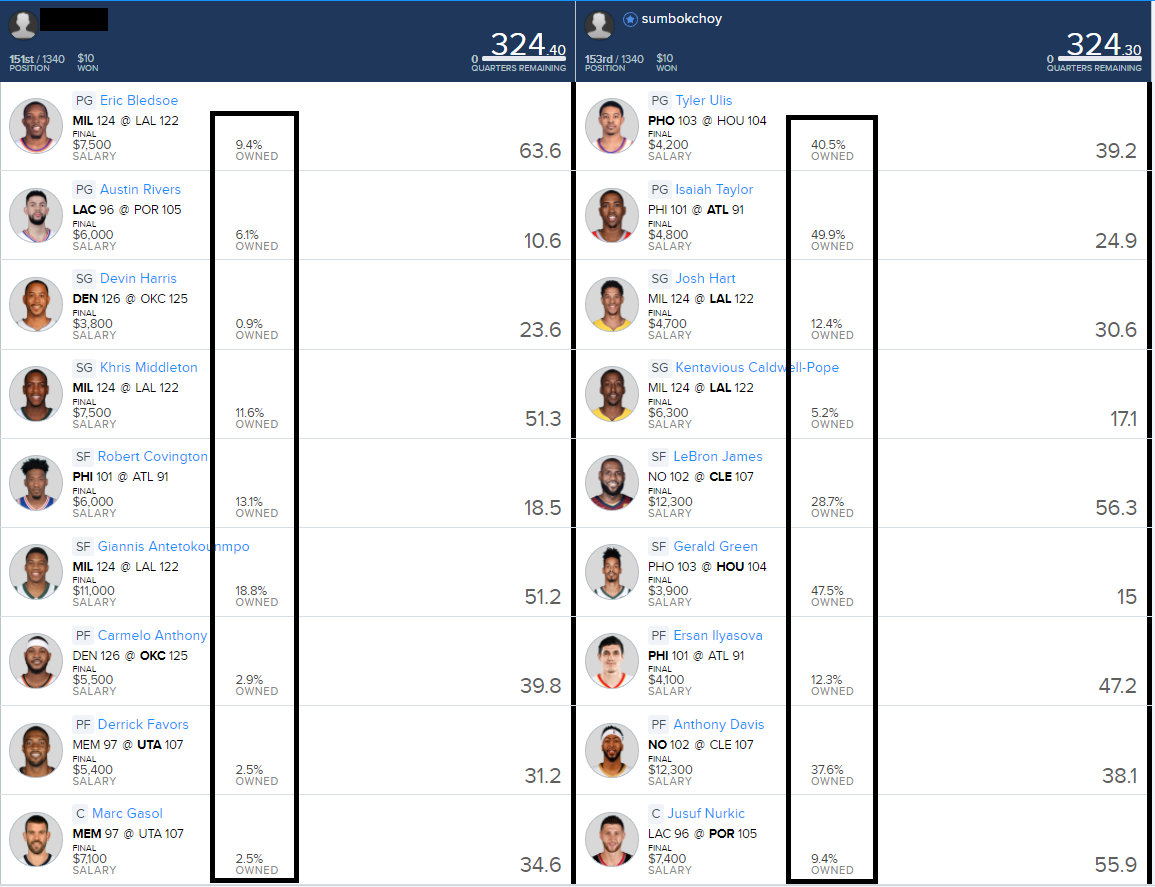
\includegraphics[width=0.8\textwidth]{figures/mevsbest}
    \caption{Good rare picks of our system versus those of a near competitor}
    \label{fig:win_record}
\end{figure}

It is also worth noting that, even in the competitions that the system does not succeed, it is still performing above average, always in the top 50th percentile. This is especially remarkable since almost all of the other competitors are marked as experienced. Competitors with a white star and blue circle have been in over 1000 competitions and have won at least \$1000 across four contests whereas competitors with a blue star and white circle have been in at least 500 competitions or have won at least \$1000 across four contests. Figure \ref{fig:competitors} shows how many of our competitors, on the winning and losing side, have these emblems. 
\begin{figure}[ht]
    \centering
    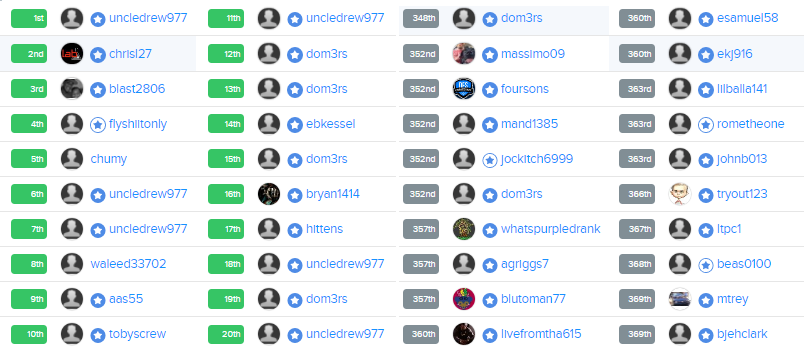
\includegraphics[width=0.6\textwidth]{figures/competitors}
    \caption{Experience level of competitors}
    \label{fig:competitors}
\end{figure}

We measured the true percentage of experienced players for a single competition, and found it to be 85\%. Our system was able to perform quite well against these experienced players, turning a profit in lineups that had all players active.However, the system is still far from being reliably profitable, as its outputs are high in variance. There are still improvements to be made.

